\section{实验}
在“基于均匀采样算法的新理论结果”一节中,我们证明了基于均匀不放回采样的算法\ref{alg: uniform_k-means}有更紧的理论界且在一定的数据假设下可以在多项式对数时间复杂度下取得常数近似的解。在本节,我们设计实验验证这一点,接受测试的基准算法分别是K-M$\text{C}^2$(算法\ref{alg:K-MC^2 seeding})和我们提出的一个新加速算法Double-K-M$\text{C}^2$,这一新算法描述见算法\ref{alg:Re-K-MC sampling},它的定位是在聚类质量和时间复杂度上位于均匀不放回采样和K-M$\text{C}^2$采样之间。这一算法提出的初衷是为了估算算法\ref{alg: reduce_k-means2}中点$s_i$上的权重$w_i$。容易知道计算准确权重需要$O(nsd)$的时间复杂度,大数据下时间复杂度太高,因此,新想法是利用一种采样算法,比如K-M$\text{C}^2$来估算权重,减少时间开销,$w_i + 1$是为了解决有的$w_i$可能是0的问题,Double-K-M$\text{C}^2$中采样部分的时间复杂度是$O(us^2 d)$,而用K-M$\text{C}^2$做基准是因为K-M$\text{C}^2$也用到了前述的假设1和2。
% remark:
% 估算方法不太对,应该乘以n/s,用Double-K-M$\text{C}^2$做基准必要性不强
\begin{algorithm}
    \caption{Double-K-M$\text{C}^2$}\label{alg:Re-K-MC sampling}
    \KwIn{数据集$\mathcal{X}$,采样数目$s$,游走次数$u$,聚类算法$\mathcal{A}_c$,类数目$k$}
    \KwOut{$k$个点$C$}
    $S_1 \gets$ 从$\mathcal{X}$中用K-M$\text{C}^2$采样$s$个点 \\
    $\mathcal{X}' \gets $ 从$\mathcal{X}$中移除$S_1$ \\
    $S_2 \gets$ 从$\mathcal{X}'$中用K-M$\text{C}^2$采样$s$个点 \\
    对$S_1$中任意点$s_i$,令$w_i$是$S_2$中离$s_i$最近的点的数目 \\
    $C \gets$ 令$w_i + 1$是$s_i$的权重,在带权的$S_1$上运行一个$\alpha$近似的算法$\mathcal{A}_c$ \\
    \textbf{返回} $C$
\end{algorithm}
这三个算法将会在八个传统聚类数据集上测试,验证他们的聚类质量和效率。另外,我们也用一个重要的实际应用-图像分割-来测试他们。在这两个任务上,结果都显示基于均匀不放回采样的算法和Double-K-M$\text{C}^2$比K-M$\text{C}^2$有更好的聚类质量而花费的时间相比K-M$\text{C}^2$又不会多太多。

\subsection{传统聚类}

\begin{table}[h]
	\caption{数据量$n$, 类数目$k$, 维度$d$}
	\label{tab:datasets}
	\begin{tabular}{cccc}
		\toprule
		数据集 & $n$ & $k$ & $d$ \\
		\midrule
		a2 & 5250 & 35 & 2 \\
		a3 & 7500 & 50 & 2 \\
		b2-random-10 & 10000 & 100 & 2 \\
		b2-random-15 & 15000 & 100 & 2 \\
		b2-random-20 & 20000 & 100 & 2 \\
		\midrule
		KDD & 145751 & 200 & 74 \\
		RNA & 488565 & 200 & 8 \\
		Poker Hand & 1000000 & 200 & 10 \\
		\bottomrule
	\end{tabular}
\end{table}

在这个任务中,我们使用五个高斯分布的合成数据集和三个大型的真实数据集(最大的数据量有100万),合成数据集\footnote{下载地址 \url{http://cs.uef.fi/sipu/datasets/}}是\textbf{a2}, \textbf{a3} (\cite{Asets}), \textbf{b2-random-10}, \textbf{b2-random-15}, \textbf{b2-random-20} (\cite{Birchsets}),真实数据集是\textbf{KDD}\footnote{下载地址 \url{http://osmot.cs.cornell.edu/kddcup/datasets.html}}(\cite{foussette2004kdd}), \textbf{RNA}\footnote{下载地址 \url{https://www.csie.ntu.edu.tw/~cjlin/libsvmtools/datasets/binary.html\#cod-rna}}(\cite{uzilov2006detection}), \textbf{Poker Hand}\footnote{下载地址 \url{https://archive.ics.uci.edu/ml/datasets/Poker+Hand}}(\cite{cattral2002evolutionary})数据集的描述参见表\ref{tab:datasets}。聚类质量用$k$-means目标函数值表示,由于代码实现会影响程序性能,所以效率/时间开销不用多少秒来评价,用计算了多少次距离来表示。

% remark
%为什么这么取值?应该用常数近似算法不应该用kmeans++,Lloyd迭代次数是多少?
算法K-M$\text{C}^2$, Double-K-M$\text{C}^2$和算法\ref{alg: uniform_k-means}的参数如下:Double-K-M$\text{C}^2$和K-M$\text{C}^2$的游走次数$u = 200$,Double-K-M$\text{C}^2$采样量$s = 1.5*\log^2 n$,算法\ref{alg: uniform_k-means}的采样量$s' = 0.7*\log^4 n$,$\alpha$近似算法是Weighted $k$-means++接上Lloyd(在算法\ref{alg: uniform_k-means}中$\alpha$近似算法的权重设为1)。所有数据集的特征都做了标准化(standardize),由于这些算法都有随机性,实验将在每个数据集上重复40次然后汇报平均值。
\begin{figure}[h]
    \subfloat[]{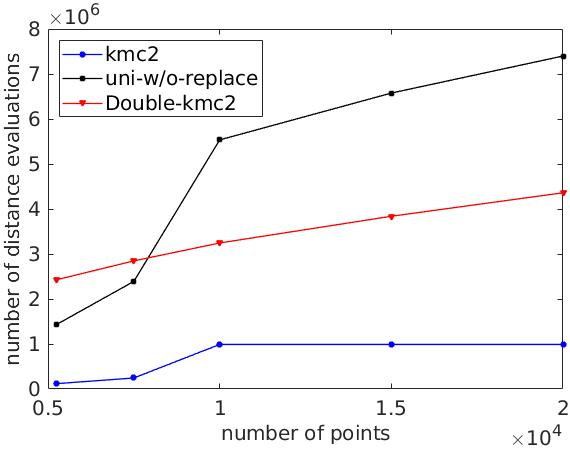
\includegraphics[width=0.49\linewidth]{syn-running-time.jpg}}
    \subfloat[]{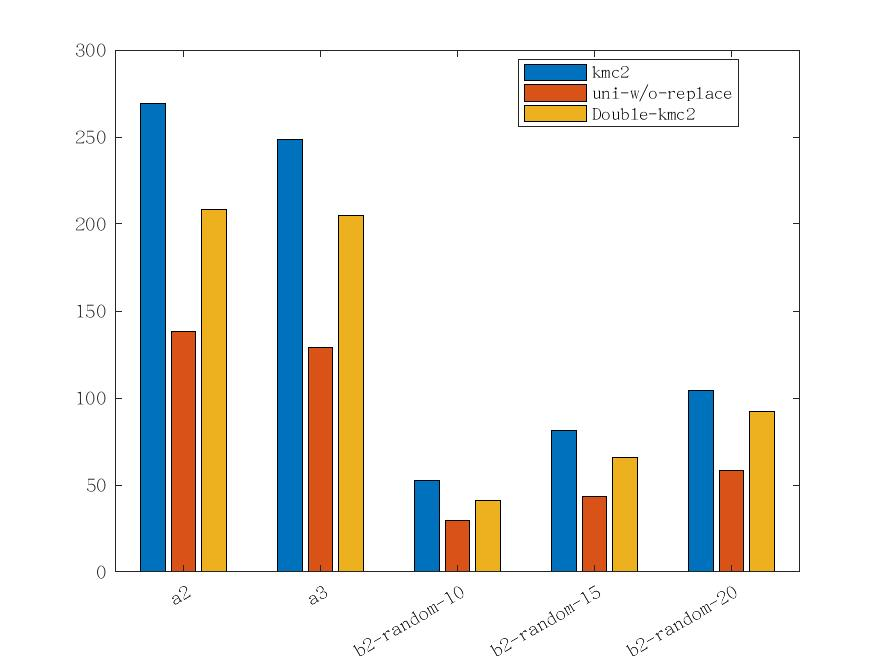
\includegraphics[width=0.49\linewidth]{syn-sum-squared-distances.jpg}} \\
    \subfloat[]{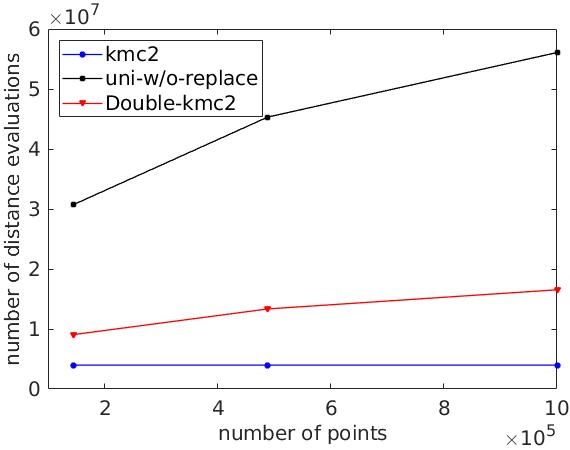
\includegraphics[width=0.49\linewidth]{real-running-time.jpg}}
    \subfloat[]{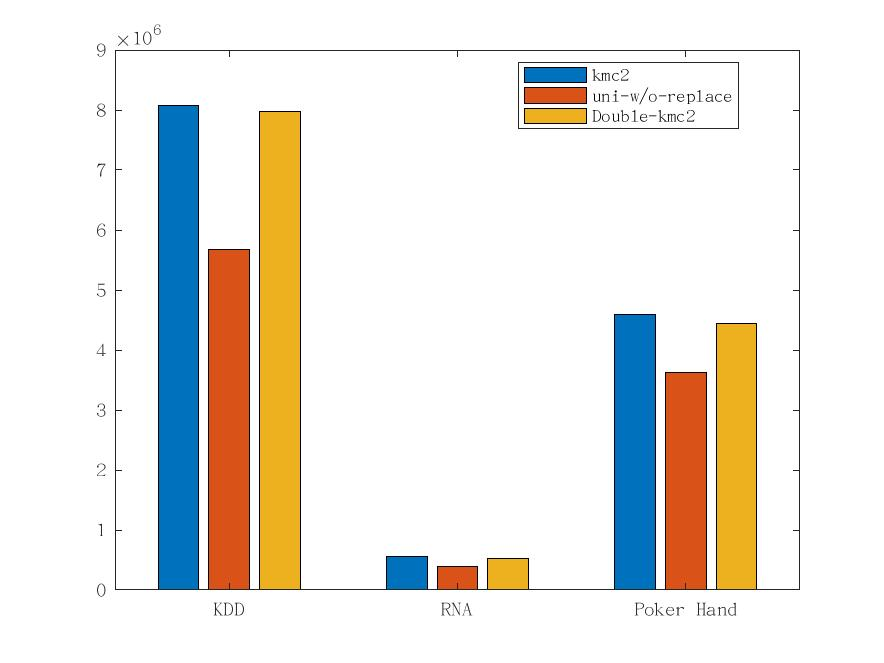
\includegraphics[width=0.49\linewidth]{real-sum-squared-distances.jpg}}
    \caption{传统聚类任务的结果。(a)合成数据集上的距离计算次数;(b)合成数据集上的$k$-means目标函数值;(c)真实数据集上的距离计算次数;(d)真实数据集上的$k$-means目标函数值}
    \label{fig: kmeans-experiments}
\end{figure}
结果见图\ref{fig: kmeans-experiments},在三个算法中基于均匀不放回采样的算法有最好的聚类效果而它的时间开销也最大,差不多是K-M$\text{C}^2$时间开销的10倍,不过随着数据量的增加,时间增加缓慢。基于均匀不放回采样的算法的$k$-means目标函数值差不多是K-M$\text{C}^2$的60\%。有意思的是,Double-K-M$\text{C}^2$的结果说明,通过K-M$\text{C}^2$采样一部分点,相比于单纯K-M$\text{C}^2$,我们能获得更好的聚类质量,而Double-K-M$\text{C}^2$的时间花费比均匀不放回要小很多。这说明,如果你倾向于一个好的聚类质量且时间开销也不想太大的话,一个好的选择是Double-K-M$\text{C}^2$,如果追求聚类质量就使用均匀不放回采样。受到特征数目和类数目的影响,$k$-means目标函数值不会随着数据量的增大而增大。图\ref{fig: kmeans-experiments}中的数据列在表\ref{tab:results on synthetic data}中,表中真实数据集上$k$-means目标函数值的数量级是$10^6$,合成数据集和真实数据集的时间开销分别在$10^6$和$10^7$数量级。

\begin{table}[h]
	\caption{传统聚类任务上$k$-means目标函数值和距离计算次数(在括号中)}
	\label{tab:results on synthetic data}
	\begin{tabular}{cccc}
		\toprule
		数据集 & K-M$\text{C}^2$ & Double-K-M$\text{C}^2$ & 基于均匀不放回采样的算法 \\
		\midrule
		% time 10^6 obj 10^0
		a2 & 269.331(0.119) & 208.395(2.428) & 138.449(1.434) \\
		a3 & 248.691(0.245) & 204.705(2.847) & 129.201(2.391) \\
		b2-random-10 & 52.358(0.990) & 41.002(3.245) & 29.519(5.536) \\
		b2-random-15 & 81.324(0.990) & 65.760(3.839) & 43.660(6.576) \\
		b2-random-20 & 104.458(0.990) & 92.411(4.361) & 58.267(7.400) \\
		\midrule % time 10^7 obj 10^7
		KDD & 8.078(0.398) & 7.978(0.908) & 5.680(3.076) \\
		RNA & 0.551(0.398) & 0.533(1.334) & 0.391(4.532) \\
		Poker Hand & 4.596(0.398) & 4.446(1.653) & 3.624(5.608) \\			
		\bottomrule
	\end{tabular}
\end{table}

\subsection{图像分割}
聚类的一个应用就是图像分割,这个应用要求对图像的不同的区块进行准确的、光滑的划分,这一应用给聚类算法聚类的质量提供了一个直观的展示。由于图像不同区块的边界不是线性的,所以需要修改$k$-means的目标函数($k$-means划分的边界是线性的),这里我们将三个算法扩展到他们对应的kernel版本。kernel $K$由以下方法构建,首先,用文献\cite{stella2003multiclass}的方法构建相似度矩阵$A$,接着,寻找一个离$A$最近的半正定矩阵$K$作为kernel,这里近与远用矩阵的Frobenius范数来度量,即求解
\begin{equation*}
	\begin{aligned}
		& \underset{K}{\text{min}} 
		& & \lVert K - A \rVert_F \\
		& s.t. 
		& & K \succeq 0
	\end{aligned}
\end{equation*}
$K \succeq 0$表示$K$是半正定矩阵。由于三个算法只返回$k$个点,$k$个划分是通过把所有点靠到离它最近的返回点上计算得到的。测试的图片是“kitten”、“bear”和“baby”\footnote{下载地址 \url{http://www.cs.utexas.edu/users/dml/Software/graclus.html}},这些图片由文献\cite{dhillon2004kernel}提供。我们调整了这些图片的长和宽,使得聚类的点的数目从900(30*30)到14400(120*120)。这个任务中kernel $k$-means的目标函数值作为聚类质量的评价指标,效率的评价指标和传统聚类中的一样。

% remark: weighted kernel kmeans++ for Double KMC^2?num of iterations?
基于均匀不放回采样的kernel版、kernel K-M$\text{C}^2$和kernel Double-K-M$\text{C}^2$的参数配置如下:均匀不放回的采样数$s' = 0.4*\log^4 n$,kernel $k$-means++是均匀不放回的$\alpha$近似算法,kernel K-M$\text{C}^2$和kernel Double-K-M$\text{C}^2$的游走次数都是200,kernel Double-K-M$\text{C}^2$的采样量是$s = 0.25*\log^2 n$,所有图片的$k$都设为5,所有算法重复30次取平均值。

\begin{figure}[h]
    \subfloat[]{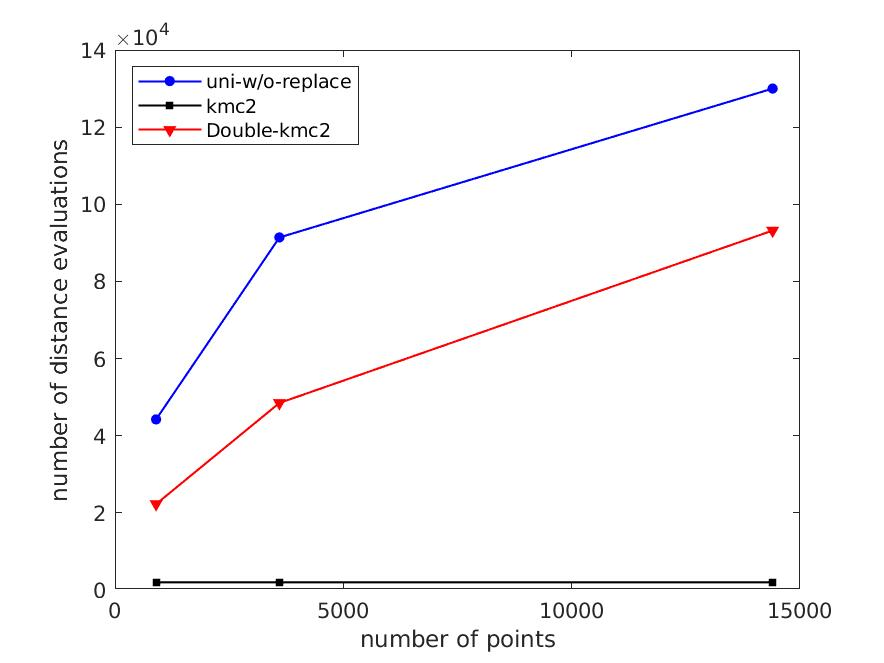
\includegraphics[width=0.49\linewidth]{image-running-time.jpg}}
    \subfloat[]{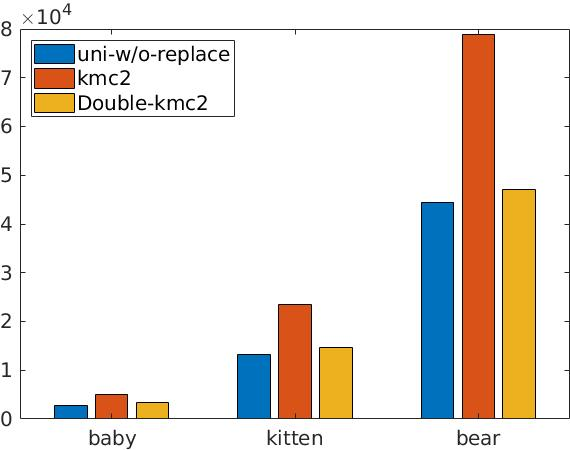
\includegraphics[width=0.49\linewidth]{image-obj.jpg}}
    \caption{图像分割任务上的结果。(a)图片数据集上的距离计算次数;(b)图片数据集上的kernel $k$-means目标函数值}
    \label{fig: image running time & ncut}
\end{figure}

% remark: 描述不量化,加上分割的图片的图,
图像分割实验结果见图\ref{fig: image running time & ncut}。实验结论和传统聚类的差不多,kernel版的均匀不放回采样有最好的聚类质量,而时间增长的趋势并不是很快,kernel Double-K-M$\text{C}^2$比均匀不放回在聚类质量上稍微差一点但是时间少了很多,kernel K-M$\text{C}^2$有最快的速度但是聚类质量太差。因此,如果你想要一个折中的平衡算法,kernel Double-K-M$\text{C}^2$是一个好的选择,如果你更关心效率,选择kernel K-M$\text{C}^2$。图\ref{fig: image running time & ncut}中的数据列在表\ref{tab:results on image segmentation}中,目标函数值的量级是$10^4$,时间开销的量级是$10^4$。
\begin{table}[h]
	\caption{图像分割任务上kernel $k$-means的目标函数值和距离计算次数(在括号中)}
	\label{tab:results on image segmentation}
	\scriptsize
	\begin{tabular}{cccc}
		\toprule
		数据集 & kernel K-M$\text{C}^2$ & kernel Double-K-M$\text{C}^2$ & 均匀不放回的kernel版 \\
		\midrule
		baby(30*30) & 0.508(0.200) & 0.341(2.228) & 0.280(4.424) \\
		kitten(60*60) & 2.345(0.200) & 1.459(4.848) & 1.323(9.140) \\
		bear(120*120) & 7.891(0.200) & 4.703(9.319) & 4.448(13.000) \\
		\bottomrule
	\end{tabular}
\end{table}
